% 2022年北京高考数学第17题：直三棱柱
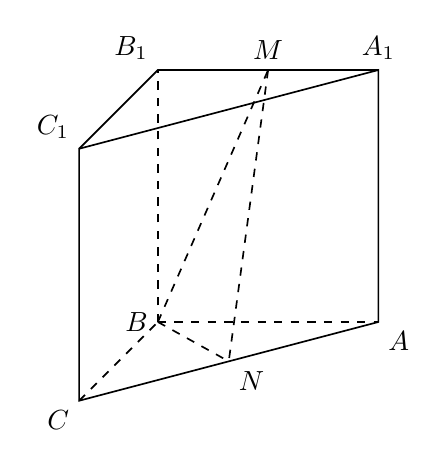
\begin{tikzpicture}[>=stealth,line width=0.6pt,font=\normalsize]
  \coordinate (C) at (0,0);
  \coordinate (A) at (3.8,1.0);
  \coordinate (B) at (1.0,1.0);
  \coordinate (C1) at (0,3.2);
  \coordinate (A1) at (3.8,4.2);
  \coordinate (B1) at (1.0,4.2);

  \coordinate (M) at (2.4,4.2);
  \coordinate (N) at (1.9,0.5);

  % 实线可见边
  \draw (C) -- (A) -- (A1) -- (C1) -- cycle;
  \draw (C1) -- (B1) -- (A1);

  % 虚线不可见边与截面线
  \draw[dashed] (C) -- (B);
  \draw[dashed] (B) -- (A);
  \draw[dashed] (B) -- (B1);
  \draw[dashed] (B) -- (M);
  \draw[dashed] (M) -- (N);
  \draw[dashed] (B) -- (N);

  % 顶点标注
  \node[below left] at (C) {$C$};
  \node[below right] at (A) {$A$};
  \node[left] at (B) {$B$};
  \node[above left] at (C1) {$C_1$};
  \node[above] at (A1) {$A_1$};
  \node[above left] at (B1) {$B_1$};
  \node[above] at (M) {$M$};
  \node[below right] at (N) {$N$};
\end{tikzpicture}
